PocketShelf is an inventory IOS/Android application. Our application consist of many features among which adding item/shelf, search item for each user with Augmented reality experience is the key feature of our application. Diagram below show the overall high level feature of our application.


\begin{figure}[h!]
	\centering
 	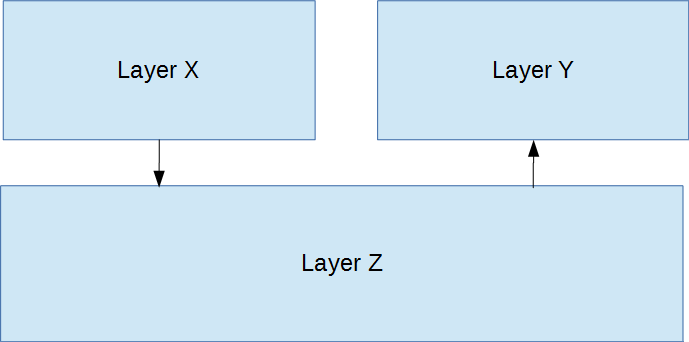
\includegraphics[width=0.60\textwidth]{images/layers}
 \caption{A simple architectural layer diagram}
\end{figure}

\subsection{Layer X Description}
Each layer should be described separately in detail. Descriptions should include the features, functions, critical interfaces and interactions of the layer. The description should clearly define the services that the layer provides. Also include any conventions that your team will use in describing the structure: naming conventions for layers, subsystems, modules, and data flows; interface specifications; how layers and subsystems are defined; etc. 

\subsection{Layer Y Description}
Each layer should be described separately in detail. Descriptions should include the features, functions, critical interfaces and interactions of the layer. The description should clearly define the services that the layer provides. Also include any conventions that your team will use in describing the structure: naming conventions for layers, subsystems, modules, and data flows; interface specifications; how layers and subsystems are defined; etc. 

\subsection{Layer Z Description}
Each layer should be described separately in detail. Descriptions should include the features, functions, critical interfaces and interactions of the layer. The description should clearly define the services that the layer provides. Also include any conventions that your team will use in describing the structure: naming conventions for layers, subsystems, modules, and data flows; interface specifications; how layers and subsystems are defined; etc. 